% ft-excel-04-LinearRegression.tex

\documentclass[xcolor=dvipsnames]{beamer}

\usepackage{cancel}
\renewcommand{\CancelColor}{\color{red}}
\usepackage{graphicx}
\usepackage{wrapfig}
\usepackage{colortbl}
\usepackage{color}
\usepackage{alltt}
\renewcommand*{\thefootnote}{\fnsymbol{footnote}}
\definecolor{myblue}{rgb}{0.8,0.85,1}

\mode<presentation>
{
  \usetheme{Warsaw}
  \setbeamercovered{transparent}
}
% \usecolortheme[named=OliveGreen]{structure}
\setbeamertemplate{navigation symbols}{} 
\setbeamertemplate{blocks}[rounded][shadow=true] 

% this is for overlaying math symbols, see https://tex.stackexchange.com/questions/12895/overlay-symbol-with-another
\def\qeq{\mathrel{%
    \mathchoice{\QEQ}{\QEQ}{\scriptsize\QEQ}{\tiny\QEQ}%
}}
\def\QEQ{{%
    \setbox0\hbox{$\longrightarrow$}%
    \rlap{\hbox to \wd0{\hss/\hss}}\box0
  }}

\newcounter{expls}
\setcounter{expls}{0}
\newcommand{\beispiel}[1]{\refstepcounter{expls}\textbf{Example \arabic{expls}: #1.}}

\newcounter{exercise}
\setcounter{exercise}{0}
\newcommand{\ubung}[0]{\refstepcounter{exercise}\textbf{Exercise \arabic{exercise}: }}

\newif\ifBCITCourse
\BCITCoursetrue
% \BCITCoursefalse
\newif\ifWhichCourse
\WhichCoursetrue
% \WhichCoursefalse
\ifBCITCourse
\ifWhichCourse
\newcommand{\CourseName}{Technical Mathematics for Food Technology}
\newcommand{\CourseNumber}{MATH 1441}
\newcommand{\CourseInst}{BCIT}
\else
\newcommand{\CourseName}{Technical Mathematics for Geomatics}
\newcommand{\CourseNumber}{MATH 1511}
\newcommand{\CourseInst}{BCIT}
\fi
\else
\newcommand{\CourseName}{Philosophy and Literature}
\newcommand{\CourseNumber}{PHIL 375}
\newcommand{\CourseInst}{UBC}
\fi

\title{Excel Functions}
\subtitle{{\CourseNumber}, BCIT}

\author{\CourseName}

\date{November 20, 2017}

\begin{document}

\begin{frame}
  \titlepage
\end{frame}

\begin{frame}
  \frametitle{Linear Regression}
  Open the file \texttt{linreg.xlsx}. These are the results of a mathematics
  aptitude tests and subsequent grades in a statistics class. Three
  students, Larry Nichols, Andrew Glosson, and Ronald Simpson ask you
  what grade they should expect to receive for their statistics class,
  given the evidence in their mathematics aptitude test (81\%, 65\%,
  and 52\%, respectively).
\end{frame}

\begin{frame}
  \frametitle{Linear Regression Screen Shot 1}
  \begin{figure}[h]
    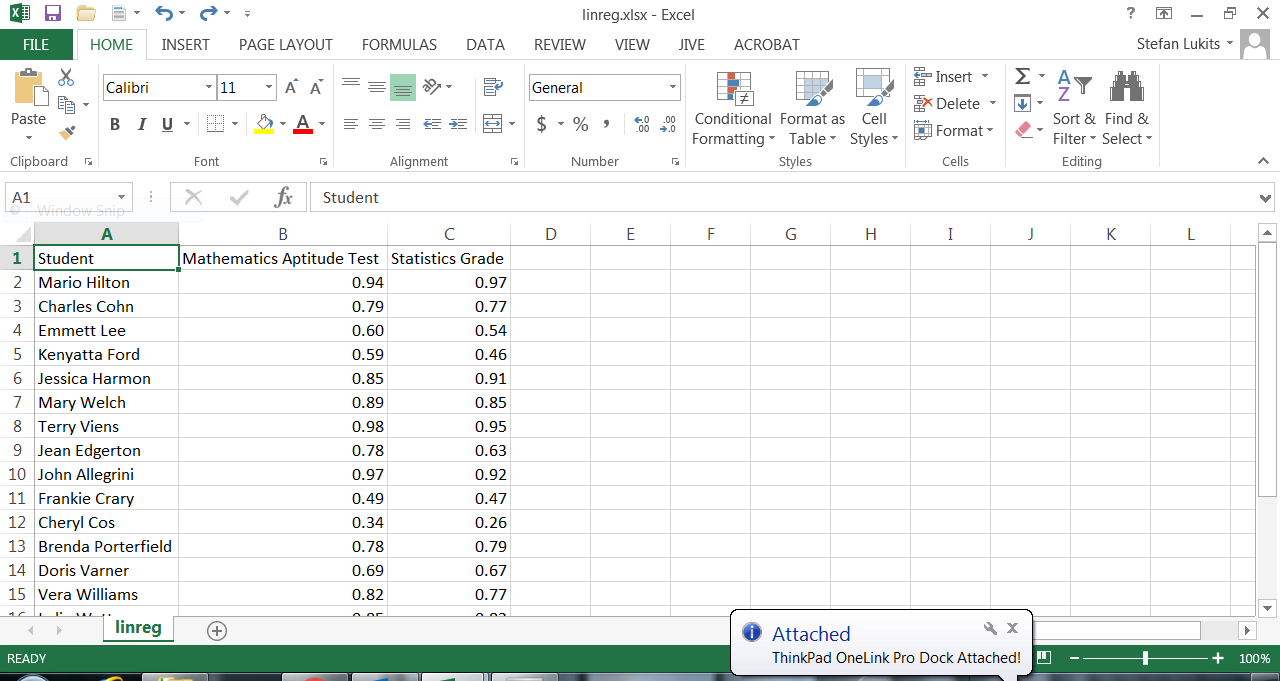
\includegraphics[scale=.42]{./linreg01.png}
  \end{figure}
\end{frame}

\begin{frame}
  \frametitle{Linear Regression Screen Shot 2}
  \begin{figure}[h]
    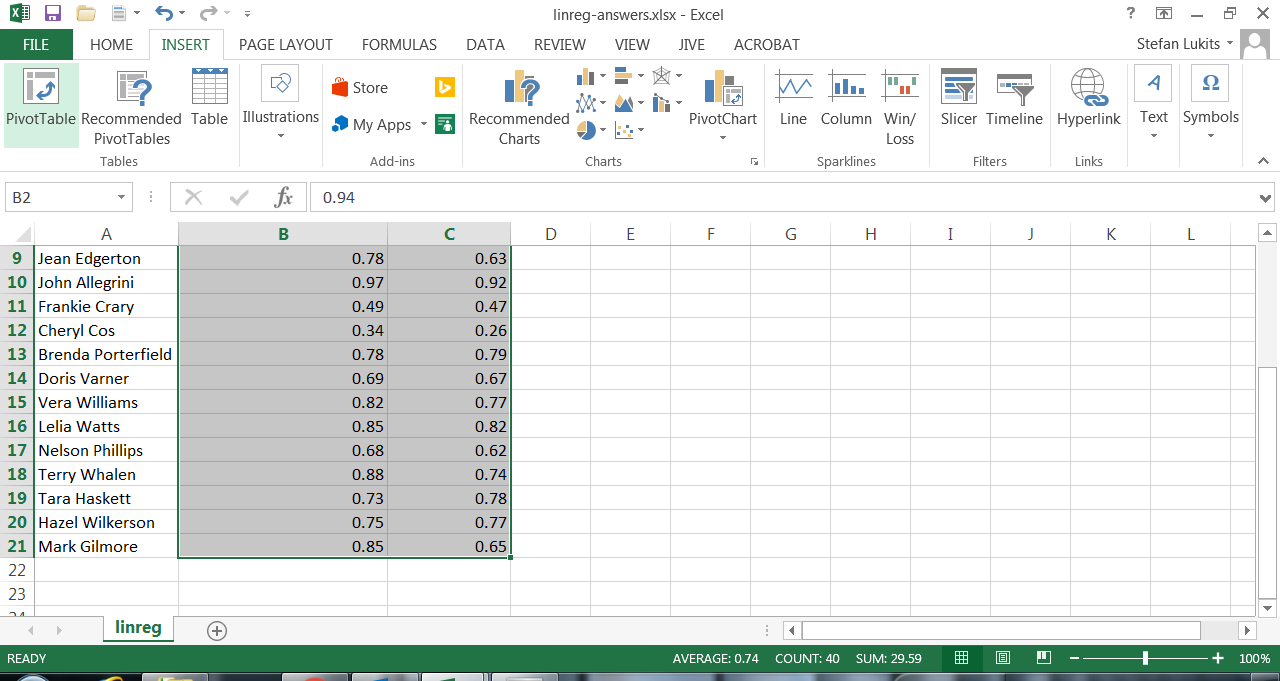
\includegraphics[scale=.42]{./linreg02.png}
  \end{figure}
\end{frame}

\begin{frame}
  \frametitle{Linear Regression Screen Shot 3}
  \begin{figure}[h]
    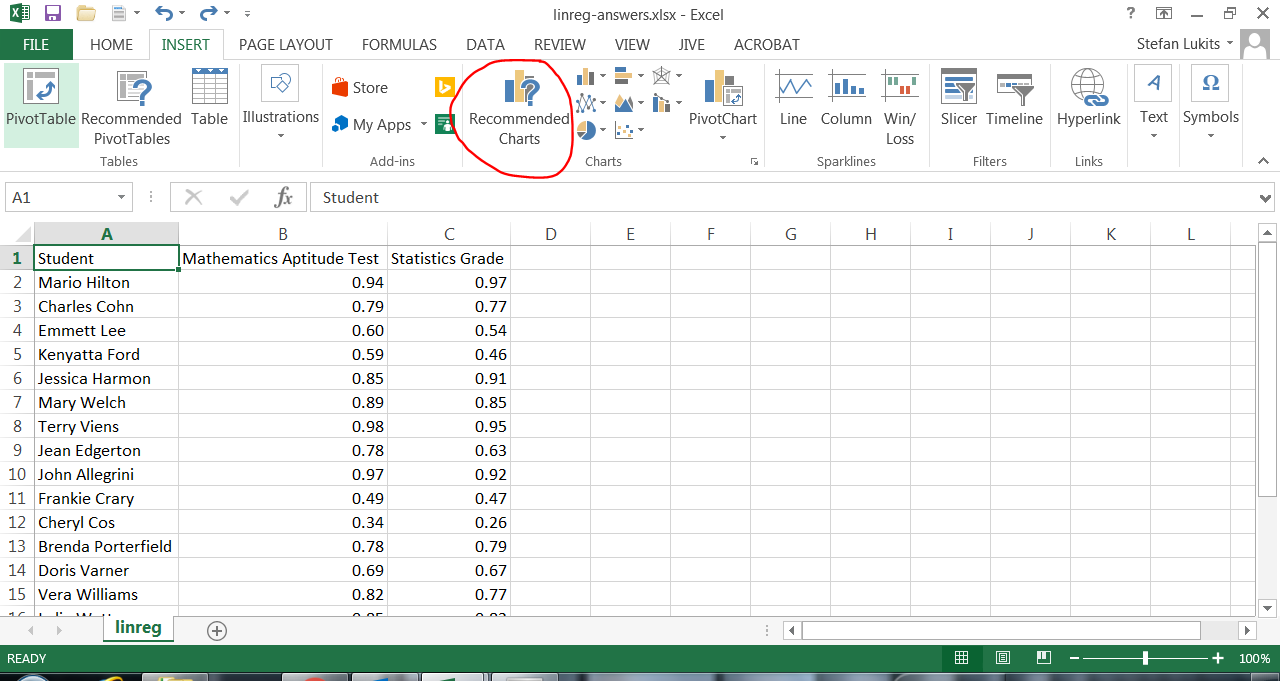
\includegraphics[scale=.42]{./linreg08.png}
  \end{figure}
\end{frame}

\begin{frame}
  \frametitle{Linear Regression Screen Shot 4}
  \begin{figure}[h]
    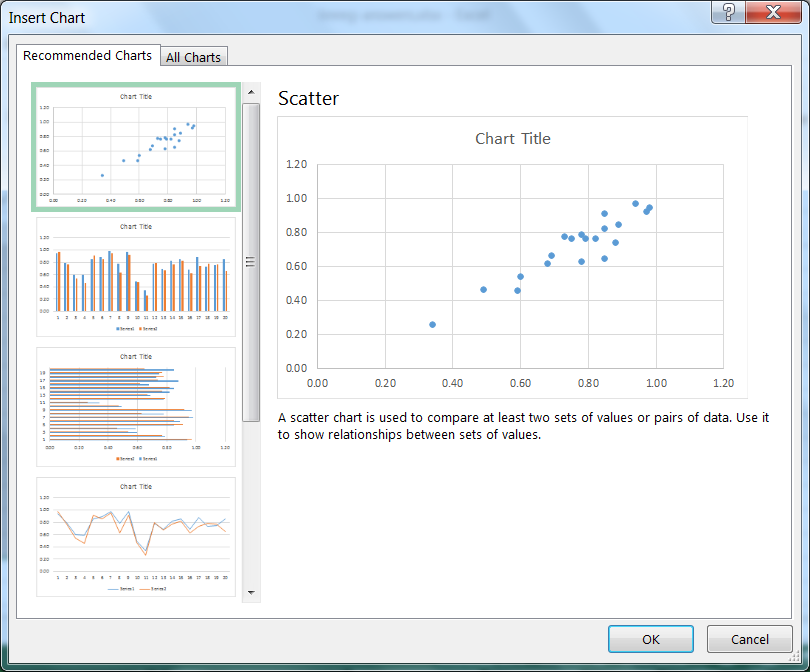
\includegraphics[scale=.42]{./linreg03.png}
  \end{figure}
\end{frame}

\begin{frame}
  \frametitle{Linear Regression Screen Shot 5}
  \begin{figure}[h]
    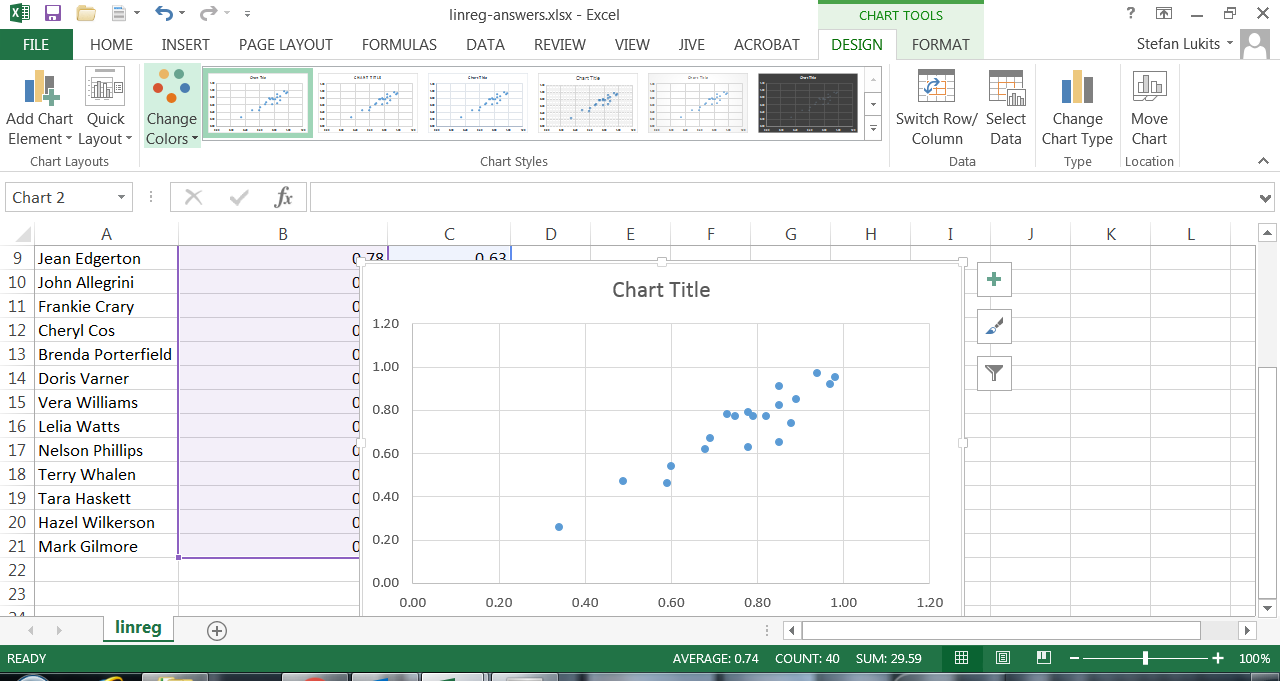
\includegraphics[scale=.42]{./linreg04.png}
  \end{figure}
\end{frame}

\begin{frame}
  \frametitle{Linear Regression Screen Shot 6}
  \begin{figure}[h]
    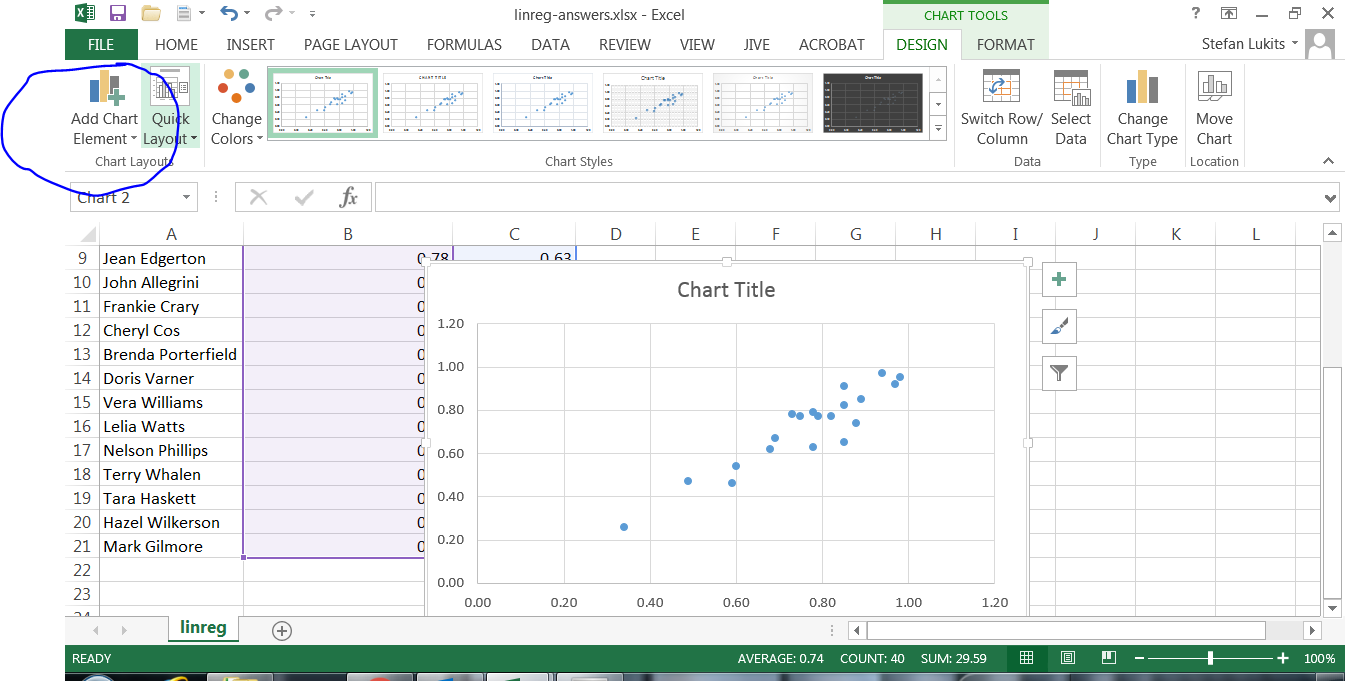
\includegraphics[scale=.42]{./linreg05.png}
  \end{figure}
\end{frame}

\begin{frame}
  \frametitle{Linear Regression Screen Shot 7}
  \begin{figure}[h]
    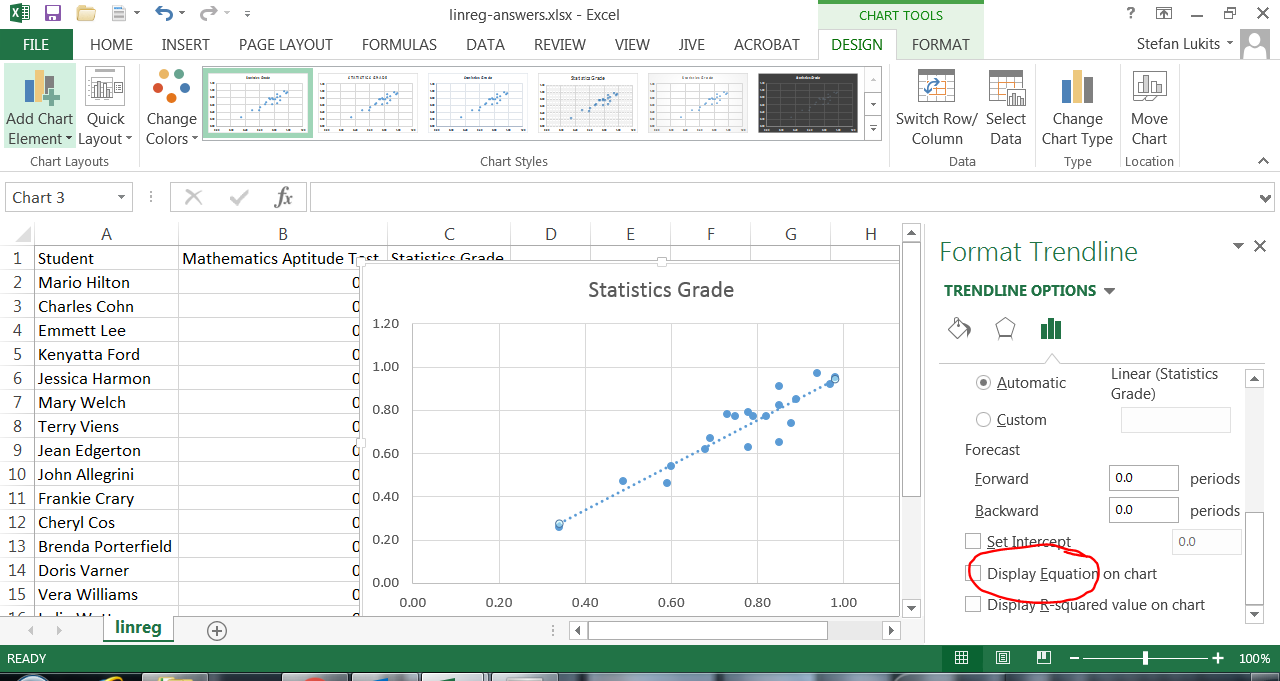
\includegraphics[scale=.42]{./linreg09.png}
  \end{figure}
\end{frame}

\begin{frame}
  \frametitle{Linear Regression Screen Shot 8}
  \begin{figure}[h]
    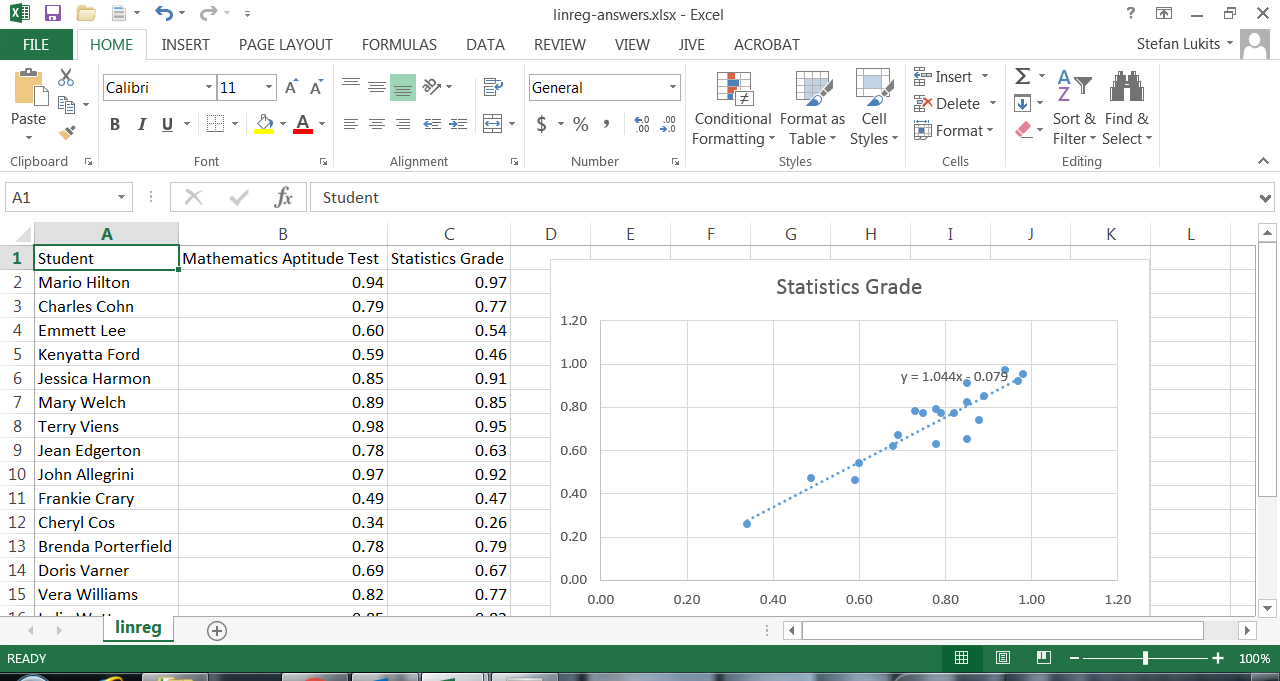
\includegraphics[scale=.42]{./linreg10.png}
  \end{figure}
\end{frame}

\begin{frame}
  \frametitle{Linear Regression Screen Shot 9}
  \begin{figure}[h]
    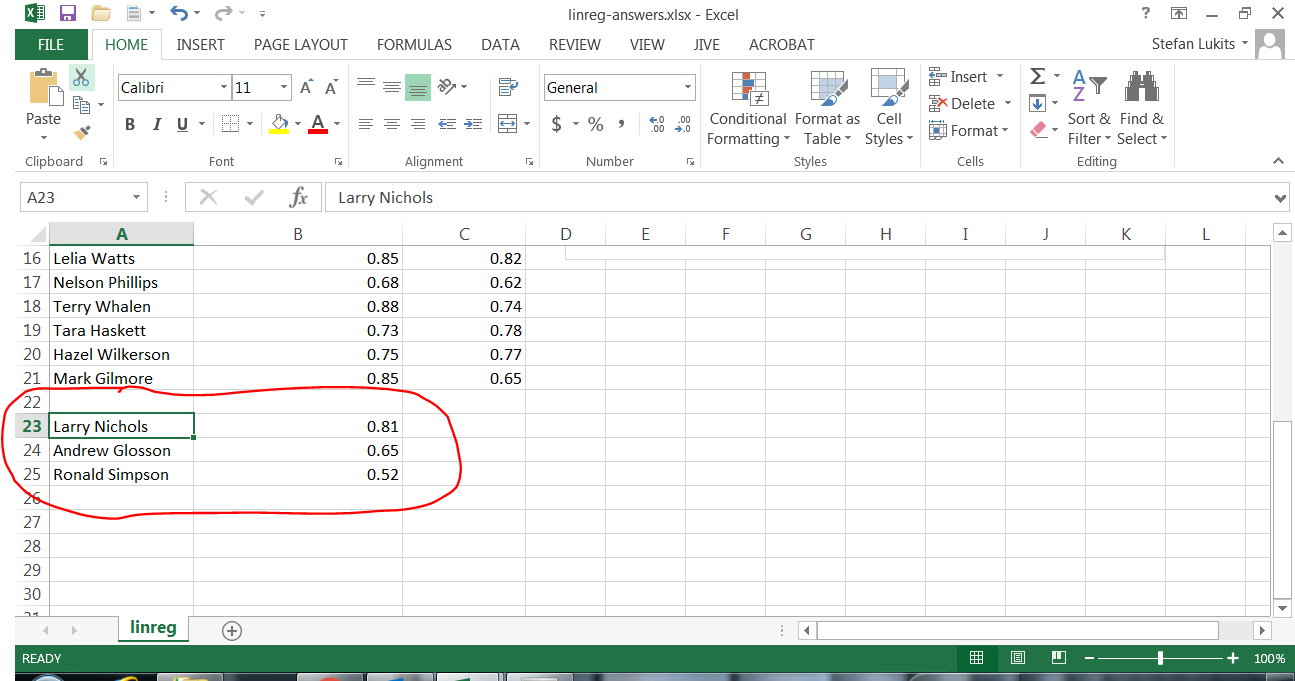
\includegraphics[scale=.42]{./linreg11.png}
  \end{figure}
\end{frame}

\begin{frame}
  \frametitle{Linear Regression Screen Shot 10}
  \begin{figure}[h]
    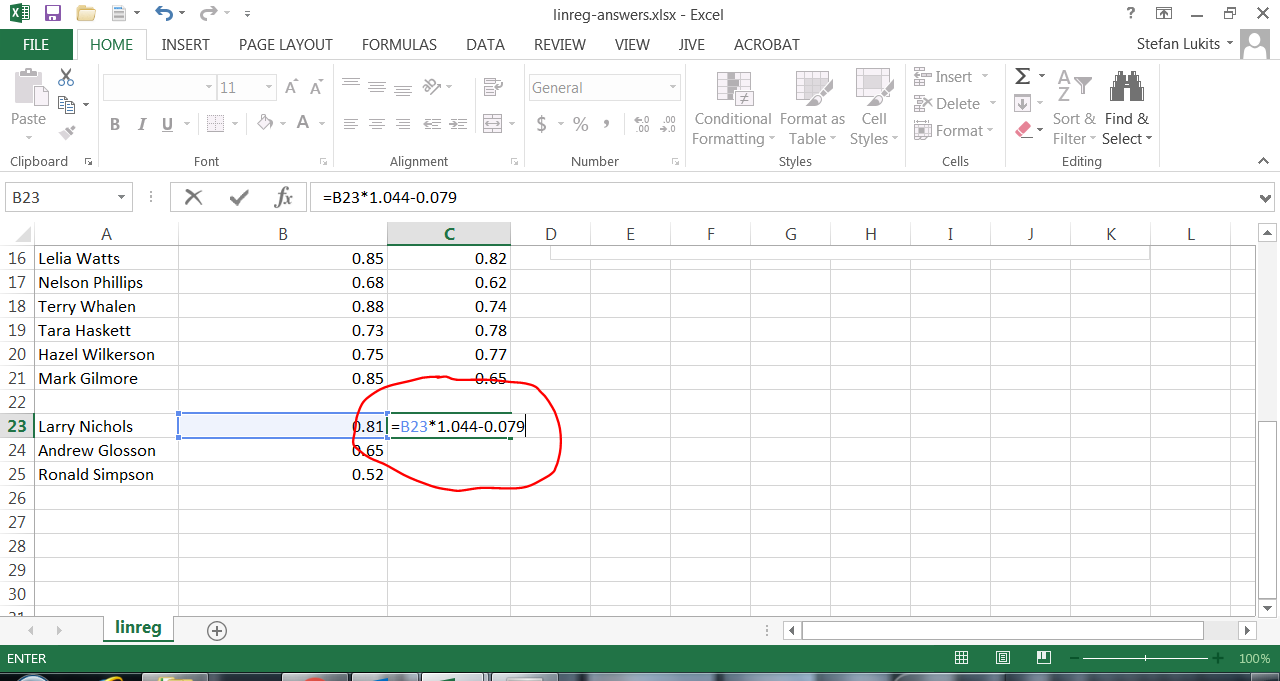
\includegraphics[scale=.42]{./linreg12.png}
  \end{figure}
\end{frame}

\begin{frame}
  \frametitle{Linear Regression Screen Shot 11}
  \begin{figure}[h]
    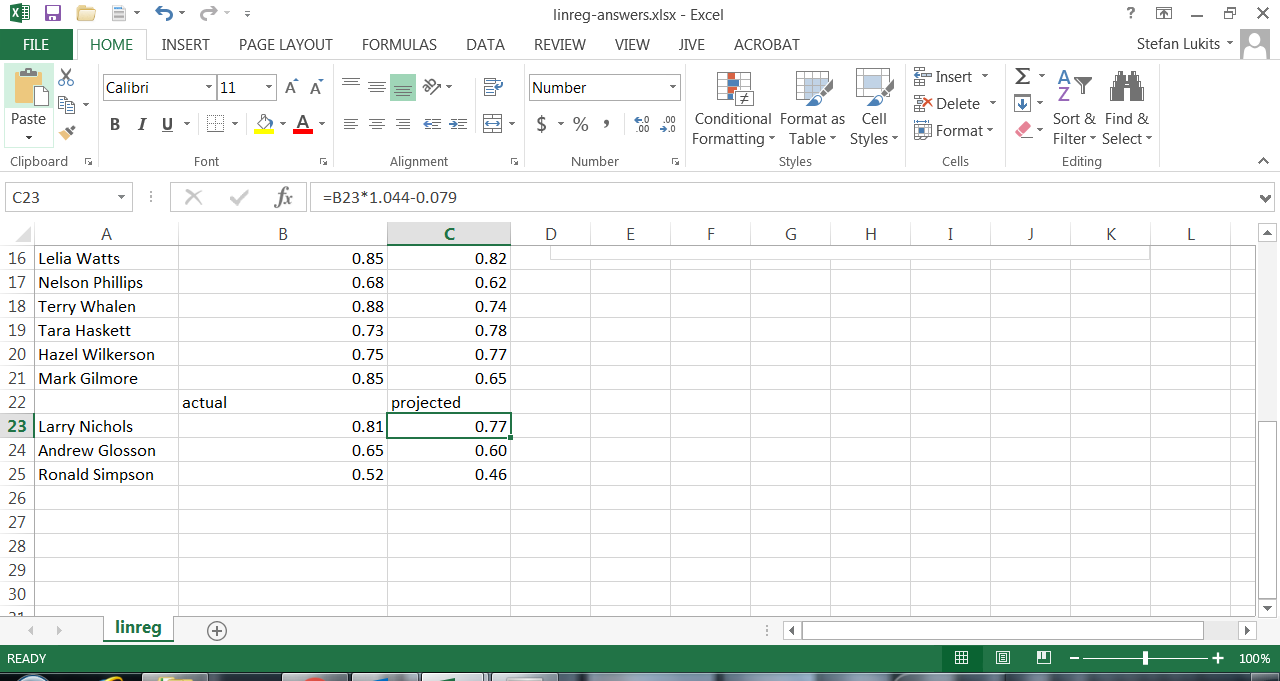
\includegraphics[scale=.42]{./linreg13.png}
  \end{figure}
\end{frame}

\begin{frame}
  \frametitle{End of Lesson}
Next Lesson: Excel Projects
\end{frame}

\end{document}

